\chapter{Musterlösung}

Alle Wireshark Mitschnitte liegen als \grqq *.pcapng \grqq{} Datei bei.

\subsection{Aufgabe 2.1 - Joining einer Phillips Hue Lampe}

\begin{figure}[H]
    \centering
    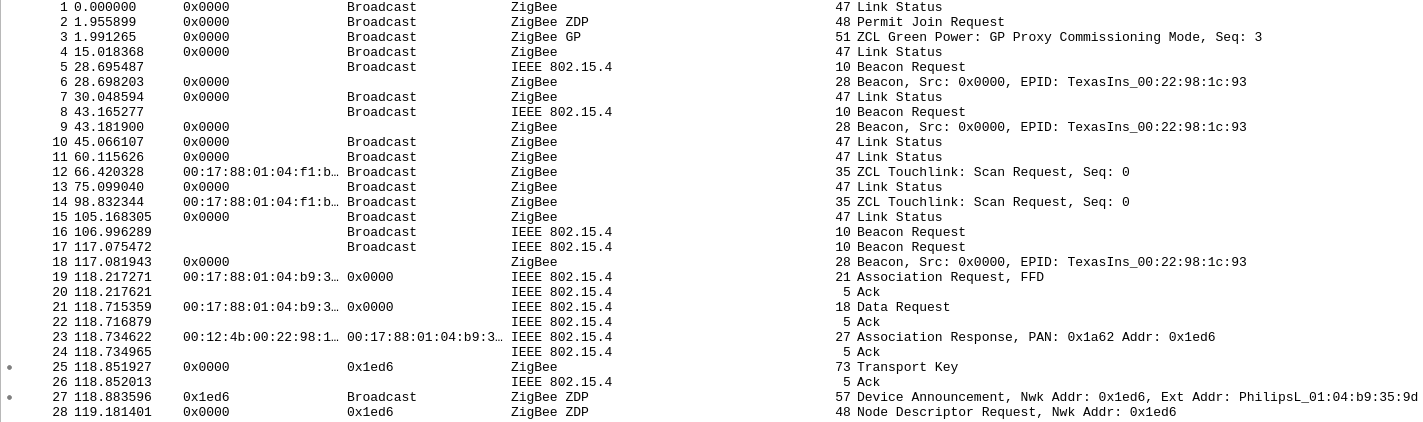
\includegraphics[width=1\textwidth]{media/lsg2.1-1.png}
    \caption{Wireshark Ausschnitt - Joining einer Lampe Teil 1}
\end{figure}

Im ersten Teil ist der Physikalische Verbindungsaufbau zu sehen. Mit Paket 2 erlaubt der Koordinator
allen Mitgliegern die Aufnahme weiterer Geräte. Paket 5 ist ein Beacon der Lampe, welcher den Beitrittswunsch
signalisiert. Auf diesen Antwortet der Koordinator jeweils mit einem Beacon Response. Nun folgt ein Association
Request sowie Data Request der Lampe (19). In der Association Response (23) bekommt die Lampe
Ihre kurze Adresse zugewiesen. In Paket 25 wird der Transport Key zur verschlüsselten Kommunikation 
übermittelt.

\begin{figure}[H]
    \centering
    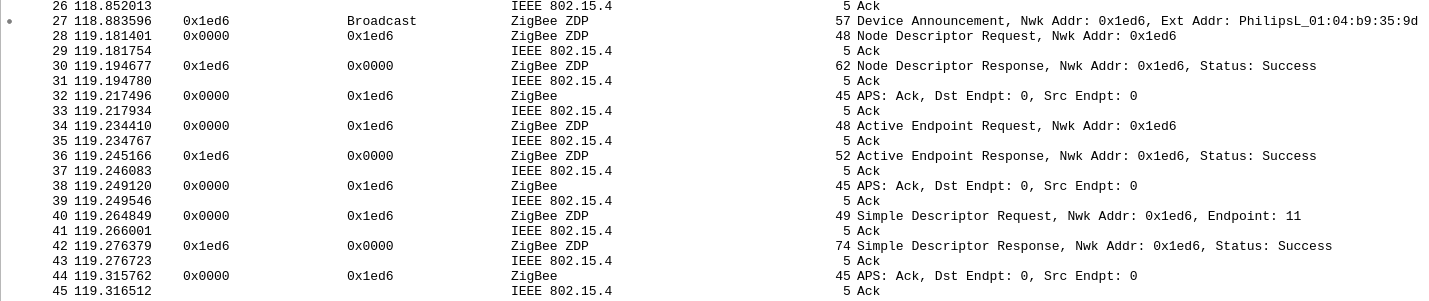
\includegraphics[width=1\textwidth]{media/lsg2.1-2.png}
    \caption{Wireshark Ausschnitt - Joining einer Lampe Teil 2}
\end{figure}

Im Anschluss fragen die Geräte gegenseitig ihre Aktiven Endpunkte über \grqq Node Descriptor\grqq{} Nachrichten ab. Die einzelnen Endpunkte werden im Anschluss per \grqq 
Active Endpoint Requests\grqq{} interviewed und per \grqq Simple Descriptor\grqq{} Nachrichten beschrieben.

\subsection{Aufgabe 2.2 - Schalten einer Lampe}

\begin{figure}[H]
    \centering
    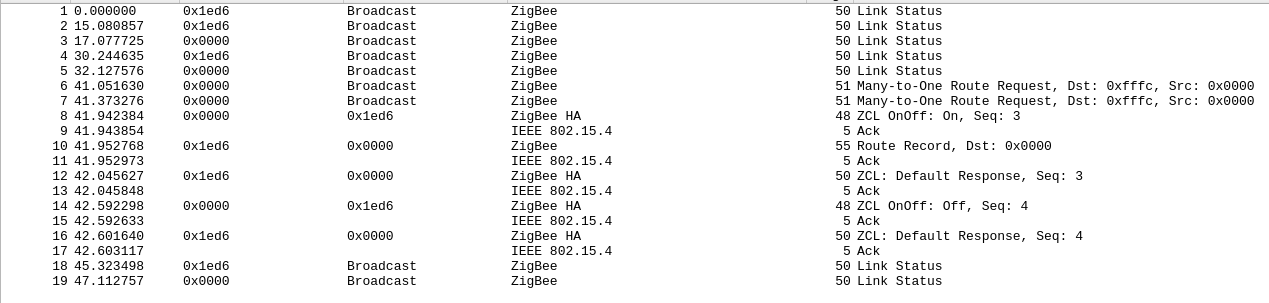
\includegraphics[width=1\textwidth]{media/lsg2.2.png}
    \caption{Wireshark Ausschnitt - Schalten einer Lampe}
\end{figure}

Hier ein ein Ein- und Auschaltvorgang einer Lampe zu sehen. Zum Schalten wird jeweils ein \grqq ZigBee Kommando Frame\grqq{} versendet, welches erst Physikalisch und 
anschließend auf ZigBee Ebene bestätigt wird.

\subsection{Aufgabe 3 - Joining einer Fernbedienung über die Lampe}

\begin{figure}[H]
    \centering
    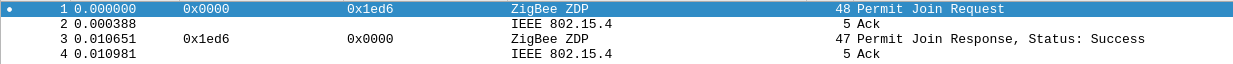
\includegraphics[width=1\textwidth]{media/lsg-3-1.png}
    \caption{Wireshark Ausschnitt - Schalten einer Lampe}
\end{figure}

Hier erteilt der Koordinator der Lampe die Erlaubniss neue Geräte in das Netzwerk aufzunehmen.

\begin{figure}[H]
    \centering
    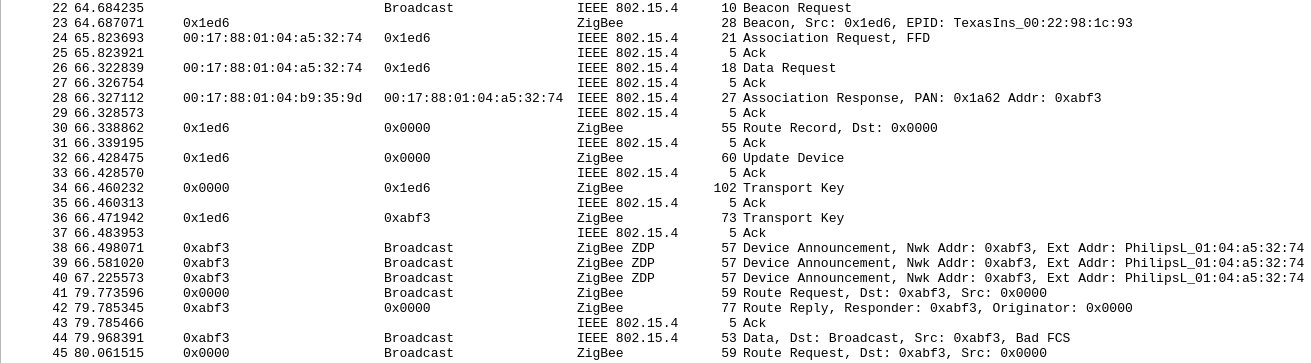
\includegraphics[width=1\textwidth]{media/lsg-3-2.png}
    \caption{Wireshark Ausschnitt - Schalten einer Lampe}
\end{figure}

Die hat zur Folge, dass die Lampe auf die Beacon-Requests der Lampe mit Beitrittswunsch reagiert. Diese Beacons dienen dazu, das Netzwerk der neuen Lampe bekannt zu machen.
Mit Nachricht 24 erfragt die neue Lampe einen Beitritt in das Netzwerk. Der Lampe wird eine Kurze Adresse sowie die PAN-ID von der Lampe im Netzwerk zugewiesen. Anschließend 
macht die bestehende Lampe das neue Gerät dem Koordinator bekannt. Dieser versendet im Anschluss den Netzwerk Schlüssel. Dieser wird in einem Tunnel verschlüsselt bis zu dem letzten
Gerät vor dem neuen Teilnehmer übermittelt. Im Anschluss erfolgt das Interview des neuen Gerätes, dies ist identisch zu Aufgabe 2.

\subsection{Aufgabe 4 - Binding der Fernbedienung}
\subsection{Aufgabe 5 - Gruppenbildung}
\subsection{Fragen}
\subsubsection{Aufgabe 2}




